\documentclass[aspectratio=169, 13pt]{beamer}
\usepackage[utf8]{inputenc}
\usepackage[brazil]{babel}
\usepackage[T1]{fontenc}
\usepackage{amsmath, amssymb, amsfonts}
\usepackage{graphicx}
\usepackage{listings}
\usepackage{xcolor}
\usepackage{booktabs}

% --- Beamer Theme & Style Configuration ---
\usetheme{Madrid}
\usecolortheme{whale}

\definecolor{geogebrablue}{RGB}{21, 101, 192}
\definecolor{geogebradark}{RGB}{13, 71, 161}
\definecolor{codebg}{RGB}{245, 247, 250}
\definecolor{codecomment}{RGB}{108, 117, 125}
\definecolor{codekw}{RGB}{198, 40, 40}
\definecolor{mathgreen}{RGB}{40, 167, 69}

\setbeamercolor{structure}{fg=geogebrablue}
\setbeamercolor{title}{fg=white, bg=geogebrablue}
\setbeamercolor{frametitle}{fg=white, bg=geogebrablue}
\setbeamercolor{block title}{fg=white, bg=geogebrablue}
\setbeamercolor{block body}{bg=codebg}
\setbeamercolor{block title example}{fg=white, bg=mathgreen}
\setbeamercolor{block body example}{bg=codebg}

\setbeamertemplate{navigation symbols}{}
\setbeamertemplate{footline}[frame number]

% Listings settings for GeoGebra Commands
\lstset{
	basicstyle=\ttfamily\footnotesize,
	backgroundcolor=\color{codebg},
	keywordstyle=\color{codekw}\bfseries,
	commentstyle=\color{codecomment}\itshape,
	stringstyle=\color{geogebrablue},
	breaklines=true,
	frame=single,
	framerule=0.5pt,
	rulecolor=\color{geogebrablue},
	showstringspaces=false
}

% --- Metadata ---
\title[Cálculo Vetorial com GeoGebra]{Cálculo Vetorial e Integrais de Linha no GeoGebra}
%\subtitle{Disciplina: Informática Aplicada ao Ensino de Matemática (5º Período)}
\author[Joao Victor]{Joao Victor}
\institute[Licenciatura em Matemática]{Graduando Licenciatura em Matemática \\ \texttt{2024007388@ifam.edu.br}}
\date{\today}

\begin{document}
	
	% -----------------------------------------------------------------------------
	% Slide 1: Title Page
	% -----------------------------------------------------------------------------
	\begin{frame}
		\titlepage
	\end{frame}
	
	% -----------------------------------------------------------------------------
	% Slide 2: Objetivos e Roteiro
	% -----------------------------------------------------------------------------
	\begin{frame}{Objetivos e Roteiro da Oficina }
		\begin{block}{Objetivo Geral}
			Articular a resolução analítica do Cálculo Vetorial com a exploração dinâmica no GeoGebra, desenvolvendo estratégias pedagógicas para o ensino superior e básico.
		\end{block}
		
		\vspace{0.2cm}
		\begin{block}{Organização do Tempo}
			\begin{enumerate}
				\item \textbf{Fundamentação e Definição 2D :} Conceitos e campo de rotação.
				\item \textbf{Cálculo Analítico e Visualização 2D :} Integral de linha e gráficos.
				\item \textbf{Prática no GeoGebra 2D :} Comandos e dinamismo.
				\item \textbf{Extensão 3D e GeoGebra 3D :} Hélice e campos no espaço.
				\item \textbf{Síntese Docente e Discussão :} Transposição didática.
			\end{enumerate}
		\end{block}
	\end{frame}
	
	% -----------------------------------------------------------------------------
	% Slide 3: Fundamentação Pedagógica
	% -----------------------------------------------------------------------------
	\begin{frame}{Fundamentação Pedagógica: O Papel do Software}
		\begin{columns}[T]
			\begin{column}{0.48\textwidth}
				\begin{block}{O Desafio no Ensino Superior}
					\begin{itemize}
						\item A transição do cálculo escalar para o vetorial exige forte intuição espacial.
						\item Fórmulas algébricas isoladas podem se tornar algoritmos desprovidos de significado.
						\item Dificuldade em visualizar vetores tangentes e circulação sobre curvas.
					\end{itemize}
				\end{block}
			\end{column}
			
			\begin{column}{0.48\textwidth}
				\begin{exampleblock}{A Contribuição do GeoGebra}
					\begin{itemize}
						\item Conecta instantaneamente as representações algébrica e gráfica.
						\item Permite simular o movimento de partículas em tempo real.
						\item Atua como um laboratório matemático para formulação de hipóteses.
					\end{itemize}
				\end{exampleblock}
			\end{column}
		\end{columns}
	\end{frame}
	
	% -----------------------------------------------------------------------------
	% Slide 4: Definição de Campo Vetorial 2D
	% -----------------------------------------------------------------------------
	\begin{frame}{Campos Vetoriais em $\mathbb{R}^2$: Conceito Formal}
		\begin{block}{Definição Matemática}
			Seja $D \subset \mathbb{R}^2$ uma região do plano. Um \textbf{campo vetorial} em $\mathbb{R}^2$ é uma função $\vec{F}$ que atribui a cada ponto $(x,y) \in D$ um vetor bidimensional:
			$$\vec{F}(x,y) = P(x,y)\,\vec{i} + Q(x,y)\,\vec{j} = \big(P(x,y),\, Q(x,y)\big)$$
			onde $P$ e $Q$ são funções escalares denominadas componentes do campo.
		\end{block}
		
		\vspace{0.2cm}
		\begin{exampleblock}{Aplicações Físicas Diretas}
			\begin{itemize}
				\item \textbf{Escoamento de Fluidos:} Vetor velocidade da água ou do ar em cada ponto.
				\item \textbf{Campos de Força:} Força gravitacional ou eletrostática atuando na região.
			\end{itemize}
		\end{exampleblock}
	\end{frame}
	
	% -----------------------------------------------------------------------------
	% Slide 5: Exemplo 2D - Formulação
	% -----------------------------------------------------------------------------
	\begin{frame}{Estudo de Caso 2D: O Campo de Rotação}
		\begin{block}{Definição do Campo}
			Consideremos o campo vetorial plano dado por:
			$$\vec{F}(x,y) = -y\,\vec{i} + x\,\vec{j} = (-y,\, x)$$
			com componentes escalares $P(x,y) = -y$ e $Q(x,y) = x$.
		\end{block}
		
		\vspace{0.3cm}
		\begin{block}{Objetivos da Investigação}
			\begin{enumerate}
				\item Analisar a relação entre o raio vetor posição $\vec{r} = (x,y)$ e o campo $\vec{F}(x,y)$.
				\item Calcular a integral de linha ao longo da circunferência unitária.
				\item Construir a representação dinâmica no GeoGebra.
			\end{enumerate}
		\end{block}
	\end{frame}
	
	% -----------------------------------------------------------------------------
	% Slide 6: Propriedade de Ortogonalidade
	% -----------------------------------------------------------------------------
	\begin{frame}{Análise Geométrica: Ortogonalidade do Campo 2D}
		\begin{block}{Produto Escalar com o Raio Vetor}
			Seja $\vec{r} = (x,y)$ o vetor posição de um ponto do plano. Efetuando o produto escalar $\vec{r} \cdot \vec{F}(x,y)$:
			$$\vec{r} \cdot \vec{F}(x,y) = (x, y) \cdot (-y, x) = -xy + xy = 0$$
		\end{block}
		
		\vspace{0.2cm}
		\begin{alertblock}{Conclusão Geométrica}
			Em qualquer ponto $(x,y) \neq (0,0)$, o vetor do campo $\vec{F}(x,y)$ é \textbf{rigorosamente ortogonal} ao vetor posição $\vec{r}$.
			\begin{itemize}
				\item As linhas de campo formam círculos concêntricos centrados na origem.
				\item A magnitude aumenta proporcionalmente à distância: $\|\vec{F}(x,y)\| = \sqrt{x^2+y^2} = r$.
			\end{itemize}
		\end{alertblock}
	\end{frame}
	
	% -----------------------------------------------------------------------------
	% Slide 7: Definição da Integral de Linha
	% -----------------------------------------------------------------------------
	\begin{frame}{Integrais de Linha de Campos Vetoriais}
		\begin{block}{Definição de Circulação / Trabalho}
			Dada uma curva suave $C$ parametrizada por $\vec{r}(t)$ para $a \le t \le b$, a integral de linha do campo $\vec{F}$ ao longo de $C$ é definida por:
			$$\int_C \vec{F} \cdot d\vec{r} = \int_{a}^{b} \vec{F}(\vec{r}(t)) \cdot \vec{r}'(t) \, dt$$
		\end{block}
		
		\vspace{0.2cm}
		\begin{exampleblock}{Significado do Integrando}
			O produto escalar $\vec{F}(\vec{r}(t)) \cdot \vec{r}'(t)$ mede a projeção do campo na direção tangente à curva:
			\begin{itemize}
				\item Se o campo aponta no mesmo sentido do movimento, a contribuição é positiva.
				\item Se for perpendicular, a contribuição instantânea é nula.
			\end{itemize}
		\end{exampleblock}
	\end{frame}
	
	% -----------------------------------------------------------------------------
	% Slide 8: Resolução Analítica 2D
	% -----------------------------------------------------------------------------
	\begin{frame}{Resolução Analítica do Exemplo 2D}
		\begin{block}{Parametrização da Trajetória}
			Circunferência unitária orientada no sentido anti-horário:
			$$\vec{r}(t) = (\cos t, \sin t), \quad t \in [0, 2\pi]$$
		\end{block}
		
		\begin{exampleblock}{Cálculo Passo a Passo}
			1. Vetor tangente/velocidade: $\vec{r}'(t) = (-\sin t, \cos t)$\\
			2. Campo sobre a curva: $\vec{F}(\vec{r}(t)) = (-\sin t, \cos t)$\\
			3. Produto escalar no integrando:
			$$\vec{F}(\vec{r}(t)) \cdot \vec{r}'(t) = (-\sin t)(-\sin t) + (\cos t)(\cos t) = \sin^2 t + \cos^2 t = 1$$
			4. Avaliação da integral:
			$$\int_C \vec{F} \cdot d\vec{r} = \int_{0}^{2\pi} 1 \, dt = 2\pi$$
		\end{exampleblock}
	\end{frame}
	
	% -----------------------------------------------------------------------------
	% Slide 9: Visualização Gráfica 2D
	% -----------------------------------------------------------------------------
	\begin{frame}{Visualização Gráfica do Campo e Trajetória 2D}
		\begin{columns}[c]
			\begin{column}{0.52\textwidth}
				\centering
				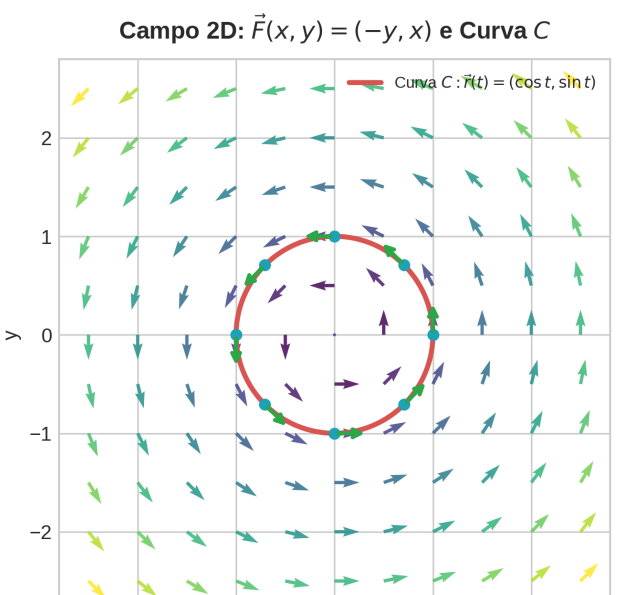
\includegraphics[height=0.68\textheight, keepaspectratio]{imagens/2d.png}
			\end{column}
			
			\begin{column}{0.45\textwidth}
				\begin{block}{Interpretação do Gráfico}
					\begin{itemize}
						\item Os vetores do campo (azul) giram ao redor da origem.
						\item Na curva $C$ (vermelho), o vetor do campo (verde) coincide exatamente com a direção tangente.
						\item Essa concordância perfeita ao longo de todo o percurso justifica o valor da integral ser $2\pi$.
					\end{itemize}
				\end{block}
			\end{column}
		\end{columns}
	\end{frame}
	
	% -----------------------------------------------------------------------------
	% Slide 10: Comandos GeoGebra 2D - Parte 1
	% -----------------------------------------------------------------------------
	\begin{frame}[fragile]{GeoGebra 2D: Comandos de Construção do Campo}
		\begin{block}{Opção A: Comando Nativo de Campo Vetorial}
			\begin{lstlisting}
				VectorField(-y, x)
			\end{lstlisting}
			Gera a malha de vetores do campo em toda a janela de visualização.
		\end{block}
		
		\begin{block}{Opção B: Construção por Componentes Escalares e Malha}
			\begin{lstlisting}
				P(x, y) = -y
				Q(x, y) = x
				grid = Sequence(Sequence(Vector((i, j), (i, j) + 0.2 (P(i, j), Q(i, j))), i, -3, 3, 1), j, -3, 3, 1)
			\end{lstlisting}
			\textbf{Explicação:}
			\begin{itemize}
				\item Definir $P$ e $Q$ isoladamente evita que o GeoGebra interprete a função como superfície.
				\item O comando \texttt{Sequence} aninhado cria a malha de amostragem.
			\end{itemize}
		\end{block}
	\end{frame}
	
	% -----------------------------------------------------------------------------
	% Slide 11: Comandos GeoGebra 2D - Parte 2
	% -----------------------------------------------------------------------------
	\begin{frame}[fragile]{GeoGebra 2D: Animação e Vetor Tangente}
		\begin{block}{Criando a Curva e o Ponto Animado}
			\begin{lstlisting}
				C = Curve(cos(t), sin(t), t, 0, 2pi)
				A = Point(C, 0.2)
			\end{lstlisting}
			Define a trajetória $C$ e um ponto $A$ vinculado a ela que pode ser animado.
		\end{block}
		
		\begin{block}{Ancorando os Vetores no Ponto}
			\begin{lstlisting}
				v_field = Vector(A, A + 0.3 (P(x(A), y(A)), Q(x(A), y(A))))
				v_tangent = TangentVector(A, C)
			\end{lstlisting}
			\textbf{Explicação:} Exibe o vetor do campo e o vetor unitário tangente atuando sobre o ponto $A$ à medida que ele se desloca sobre a curva.
		\end{block}
	\end{frame}
	
	% -----------------------------------------------------------------------------
	% Slide 12: Definição de Campo Vetorial 3D
	% -----------------------------------------------------------------------------
	\begin{frame}{Campos Vetoriais em $\mathbb{R}^3$: Extensão Espacial}
		\begin{block}{Definição Formal}
			Um \textbf{campo vetorial em $\mathbb{R}^3$} associa a cada ponto $(x,y,z) \in E \subset \mathbb{R}^3$ um vetor tridimensional:
			$$\vec{F}(x,y,z) = P(x,y,z)\,\vec{i} + Q(x,y,z)\,\vec{j} + R(x,y,z)\,\vec{k}$$
		\end{block}
		
		\vspace{0.2cm}
		\begin{exampleblock}{Integral de Linha no Espaço Tridimensional}
			Para uma curva $C$ parametrizada por $\vec{r}(t) = (x(t), y(t), z(t))$, para $t \in [a,b]$:
			$$\int_C \vec{F} \cdot d\vec{r} = \int_{a}^{b} \Big[ P(\vec{r}(t))x'(t) + Q(\vec{r}(t))y'(t) + R(\vec{r}(t))z'(t) \Big] dt$$
		\end{exampleblock}
	\end{frame}
	
	% -----------------------------------------------------------------------------
	% Slide 13: Exemplo 3D - Formulando o Campo Helicoidal
	% -----------------------------------------------------------------------------
	\begin{frame}{Estudo de Caso 3D: Campo Helicoidal e a Hélice}
		\begin{block}{Definição do Campo e da Trajetória}
			Consideremos o campo tridimensional e a curva hélice $C$:
			$$\vec{F}(x,y,z) = (-y, x, 1), \quad \vec{r}(t) = (\cos t, \sin t, t), \quad t \in [0, 2\pi]$$
		\end{block}
		
		\vspace{0.2cm}
		\begin{block}{Características Geométricas}
			\begin{itemize}
				\item No plano $xy$, as componentes $(-y, x)$ promovem rotação anti-horária.
				\item A componente $z = 1$ adiciona um vetor vertical constante para cima.
				\item A curva combina rotação circular com elevação linear constante.
			\end{itemize}
		\end{block}
	\end{frame}
	
	% -----------------------------------------------------------------------------
	% Slide 14: Resolução Analítica 3D
	% -----------------------------------------------------------------------------
	\begin{frame}{Resolução Analítica do Exemplo 3D}
		\begin{block}{Cálculo da Integral de Linha no Espaço}
			Dada a hélice $\vec{r}(t) = (\cos t, \sin t, t)$ para $t \in [0, 2\pi]$:
		\end{block}
		
		\begin{exampleblock}{Passos do Cálculo}
			1. Derivada da hélice: $\vec{r}'(t) = (-\sin t, \cos t, 1)$\\
			2. Campo avaliado na curva: $\vec{F}(\vec{r}(t)) = (-\sin t, \cos t, 1)$\\
			3. Produto escalar:
			$$\vec{F}(\vec{r}(t)) \cdot \vec{r}'(t) = (-\sin t)(-\sin t) + (\cos t)(\cos t) + (1)(1) = 1 + 1 = 2$$
			4. Resultado da Integral:
			$$\int_C \vec{F} \cdot d\vec{r} = \int_{0}^{2\pi} 2 \, dt = 4\pi$$
		\end{exampleblock}
	\end{frame}
	
	% -----------------------------------------------------------------------------
	% Slide 15: Visualização Gráfica 3D
	% -----------------------------------------------------------------------------
	\begin{frame}{Visualização Gráfica 3D: Hélice e Campo Espacial}
		\begin{columns}[c]
			\begin{column}{0.52\textwidth}
				\centering
				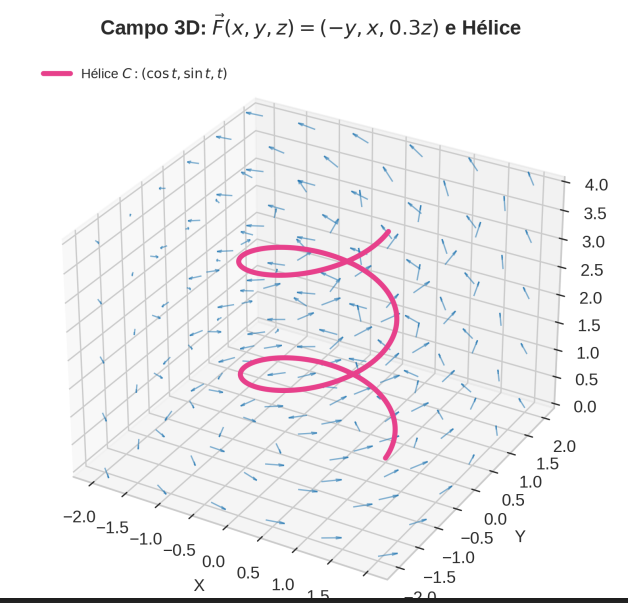
\includegraphics[height=0.68\textheight, keepaspectratio]{imagens/3d.png}
			\end{column}
			
			\begin{column}{0.45\textwidth}
				\begin{block}{Análise no Espaço}
					\begin{itemize}
						\item A curva em vermelho representa a hélice subindo de $z=0$ até $z=2\pi$.
						\item Os vetores do campo acompanham tanto o giro horizontal quanto a subida vertical.
						\item O valor obtido ($4\pi$) traduz o trabalho total realizado pelo campo durante a ascensão.
					\end{itemize}
				\end{block}
			\end{column}
		\end{columns}
	\end{frame}
	
	% -----------------------------------------------------------------------------
	% Slide 16: Comandos GeoGebra 3D
	% -----------------------------------------------------------------------------
	\begin{frame}[fragile]{GeoGebra 3D: Comandos na Janela 3D}
		\begin{block}{1. Definindo a Hélice}
			\begin{lstlisting}
				Helix = Curve(cos(t), sin(t), t, t, 0, 2pi)
			\end{lstlisting}
		\end{block}
		
		\begin{block}{2. Componentes Escalares do Campo 3D}
			\begin{lstlisting}
				P3(x, y, z) = -y
				Q3(x, y, z) = x
				R3(x, y, z) = 1
			\end{lstlisting}
		\end{block}
		
		\begin{block}{3. Malha de Vetores sobre a Hélice}
			\begin{lstlisting}
				vectors3D = Sequence(Vector(Helix(t), Helix(t) + 0.3 (P3(x(Helix(t)), y(Helix(t)), z(Helix(t))), Q3(x(Helix(t)), y(Helix(t)), z(Helix(t))), R3(x(Helix(t)), y(Helix(t)), z(Helix(t))))), t, 0, 2pi, pi/4)
			\end{lstlisting}
		\end{block}
	\end{frame}
	
	% -----------------------------------------------------------------------------
	% Slide 17: Campos Conservativos e Gradiente
	% -----------------------------------------------------------------------------
	\begin{frame}{Aplicação Especial: Campos Gradiente e Conservativos}
		\begin{block}{Teorema Fundamental das Integrais de Linha}
			Se $\vec{F} = \nabla f$ for um campo conservativo derivado de um potencial escalar $f$, então:
			$$\int_C \nabla f \cdot d\vec{r} = f(\vec{r}(b)) - f(\vec{r}(a))$$
			A integral de linha independe do caminho, dependendo apenas dos pontos inicial e final.
		\end{block}
		
		\vspace{0.2cm}
		\begin{exampleblock}{Propriedade da Ortogonalidade}
			O vetor gradiente $\nabla f(x,y)$ é sempre \textbf{ortogonal às curvas de nível} $f(x,y) = k$.
		\end{exampleblock}
	\end{frame}
	
	% -----------------------------------------------------------------------------
	% Slide 18: GeoGebra - Curvas de Nível
	% -----------------------------------------------------------------------------
	\begin{frame}[fragile]{GeoGebra: Curvas de Nível e Gradiente}
		\begin{block}{Comandos no GeoGebra}
			\begin{lstlisting}
				f(x, y) = x^2 y - y^3
				levels = ContourPlot(f, -4, 4, 0.5)
				GradX(x, y) = 2 x y
				GradY(x, y) = x^2 - 3 y^2
				gradGrid = Sequence(Sequence(Vector((i, j), (i, j) + 0.15 (GradX(i, j), GradY(i, j))), i, -3, 3, 1), j, -3, 3, 1)
			\end{lstlisting}
		\end{block}
		
		\begin{exampleblock}{Exploração Visual em Sala}
			Ao projetar essa construção, a turma verifica imediatamente que os vetores do gradiente cortam as linhas de nível em ângulos de $90^\circ$.
		\end{exampleblock}
	\end{frame}
	
	% -----------------------------------------------------------------------------
	% Slide 19: Transposição Didática
	% -----------------------------------------------------------------------------
	\begin{frame}{Transposição Didática no Ensino de Matemática}
		\begin{block}{Reflexões para a Ação Docente}
			\begin{itemize}
				\item \textbf{Aprendizagem Ativa:} Promover momentos em que os alunos manipulem parâmetros no GeoGebra em vez de apenas assistir à exposição.
				\item \textbf{Conexão Múltipla:} Alternar de forma consciente entre a álgebra das integrais e a geometria dos vetores.
				\item \textbf{Investigação de Erros:} Utilizar inconsistências visuais para diagnosticar falhas na parametrização ou nos limites de integração.
			\end{itemize}
		\end{block}
	\end{frame}
	
	% -----------------------------------------------------------------------------
	% Slide 20: Considerações Finais
	% -----------------------------------------------------------------------------
	\begin{frame}{Considerações Finais}
		\begin{block}{Síntese da Oficina}
			\begin{itemize}
				\item A integração entre cálculo analítico e ferramentas dinâmicas fortalece o rigor e a intuição.
				\item O uso de comandos estruturados no GeoGebra desenvolve o pensamento computacional dos licenciandos.
				\item A abordagem bidimensional e tridimensional prepara os futuros professores para o ensino da matemática contemporânea.
			\end{itemize}
		\end{block}
		
		\vspace{0.4cm}
		\centering
		\Large\textbf{\color{geogebrablue} Muito Obrigado!}\\
		\small Perguntas e Discussão
	\end{frame}
	
\end{document}
